\documentclass[12pt, catalan]{article}

\usepackage[utf8]{inputenc}
\usepackage[T1]{fontenc}
\usepackage{babel}
\usepackage{lmodern}
\usepackage{geometry}
\usepackage{hyperref}
\usepackage[dvipsnames]{xcolor}
\usepackage[sf,bf,small,pagestyles]{titlesec}
\usepackage{titling}
\usepackage[font={footnotesize, sf}, labelfont=bf]{caption} 
\usepackage{siunitx}
\usepackage{graphicx}
\usepackage{subfigure}
\usepackage{tikz}
\usepackage{multirow}
\usepackage{booktabs}
\usepackage{amsmath,amssymb}
\usepackage{mathtools}
\usepackage[sort]{cleveref}
\usepackage{enumitem}

% Configuració dels marges
\geometry{
	a4paper,
	right = 2.5cm,
	left = 2.5cm,
	bottom = 3cm,
	top = 3cm
}

% Configuració dels links i referències
\hypersetup{
	colorlinks,
	linkcolor = {red!50!blue},
	linktoc = page
}

\crefname{figure}{figura}{figures}
\crefname{table}{taula}{taules}
\numberwithin{table}{section}
\numberwithin{figure}{section}
\numberwithin{equation}{section}

% Unitats
\sisetup{
	inter-unit-product = \ensuremath{ \, },
	allow-number-unit-breaks = true,
	math-celsius = {}^{\circ}\kern-\scriptspace C,
	detect-family = true,
	detect-shape = true,
	list-final-separator = { i },
	list-pair-separator = { i },
	list-units = single,
	separate-uncertainty = true
}
\renewcommand{\arraystretch}{1}
\newcommand{\param}[2]{\multicolumn{5}{c}{\( #1 = #2 \)}}
\newcommand{\paramnu}[1]{{\( \nu = #1 \)}}

\newpagestyle{pagina}{
	\headrule
	\sethead*{\sffamily \small {\bfseries Comparació d'estimadrors}}{}{\small \sffamily \theauthor}
	\footrule
	\setfoot*{}{}{\small \sffamily \thepage}
}
\pagestyle{pagina}

% Nous comands
\newcommand{\cond}{\, \vert \,}
\renewcommand{\L}{\mathcal{L}}
\DeclareMathOperator{\DGamma}{Gamma}
\DeclareMathOperator{\MSE}{MSE}
\DeclareMathOperator{\RMSE}{RMSE}
\DeclareMathOperator{\E}{\mathbb{E}}
\DeclareMathOperator{\Var}{Var}
\newcommand{\abs}[1]{\left|#1\right|}

\title{\sffamily \bfseries Comparació d'estimadors}
\author{\sffamily Andreu Arderiu, Arnau Mas, Alejandro Plaza}
\date{24 d'Abril de 2019}

\begin{document}

\maketitle

\begin{abstract}
    L'objectiu d'aquest treball és calcular els estimadors dels paràmetres de la distribució gamma mitjançant el mètode dels moments i màxima versemblança, i comparar la seva validesa segons el mètode usat. 
   Així doncs, simularem mostres de dades distribuïdes segons una gamma de paràmetres fixats, i estudiarem la consistència, biaix i error quadràtic mig dels estimadors obtinguts. D'aquesta manera, analitzarem com varien aquestes magnituds en funció de la mida mostral de les dades, dels valors dels paràmetres de la distribució gamma, i del mètode usat per a calcular els estimadors.\vspace{0.5cm}\\
   The goal of this assignment is to compute the estimators for the parameters of the gamma distribution with the method of moments and the method of maximum likelihood estimation (MLE).
   To do so, we will simulate data samples that follow a gamma distribution with fixed parameters, and we will study the consistency, bias, and mean squared error (MSE) of the estimators obtained. Indeed, we will analyze the variation of these magnitudes with respect to the sample size, the gamma distribution parameter's values chosen, and the method used to calculate the estimators.
\end{abstract}

\section{Introducció i conceptes preliminars}
La funció de densitat d'una variable aleatòria \( X \) que segueix la distribució gamma és:
\begin{equation*}
	f_X(x \cond \alpha, \nu) = \frac{\alpha^\nu x^{\nu - 1}}{\Gamma(\nu)} e^{-\alpha x},
\end{equation*}
on \( \alpha \) i \( \nu \) són paràmetres positius que s'anomenen de ràtio (\emph{rate} en anglès) i de forma (\emph{shape} en anglès), respectivament. El nostre objectiu és produir estimadors per aquests dos paràmetres mitjançant els mètodes de màxima versemblança i dels moments i comparar-los.  

\subsection{Mètode dels moments}
La funció generatriu de moments d'una variable aleatòria de distribució gamma, \( X \sim \DGamma(\alpha, \nu) \) és
\begin{equation*}
	M_X(t) = \alpha^\nu (\alpha - t)^{-\nu },
\end{equation*}
i les successives derivades són:
\begin{align*}
	M'_X(t) &= \nu \alpha^\nu (\alpha - t)^{-\nu - 1}, \\
	M''_X(t) &= \nu(\nu + 1) \alpha^\nu (\alpha - t)^{-\nu - 2}. 
\end{align*}
Per tant, per la definició de la funció generatriu tenim:
\begin{align} 
		\E[X] &= M'_X(0) = \frac{\nu}{\alpha}\label{e}, \\
		\Var[X] &= \E[X^2] - \E[X]^2 = M''_X(0) - M'_X(0)^2 = \frac{\nu(\nu + 1)}{\alpha^2} - \left( \frac{\nu}{\alpha} \right)^2 = \frac{\nu}{\alpha^2}. \label{var}
\end{align}
Aïllant $\alpha$ i $\nu$ en les expressions (\ref{e}), (\ref{var})  obtenim:
\begin{align} 
		\alpha &= \frac{\E[X]}{\Var[X]}\label{alpha1},\\
		\nu &= \frac{\E[X]^2}{\Var[X]}. \label{nu1}.
\end{align}
Així, si tenim una mostra $\mathbf{X} = \left\{X_1, \dots, X_n\right\}$, on les $X_i$ són variables aleatòries idènticament distribuïdes segons la distribució del model $X$, aleshores els estimadors per als paràmetres que obtenim amb el mètode dels moments són:
\begin{align*}
	\hat{\alpha}_\text{mom}(\mathbf{X}) &= \frac{\bar{X}}{S^2}, \\
	\hat{\nu}_\text{mom}(\mathbf{X}) &= \frac{\bar{X}^2}{S^2}, 
\end{align*}
on \( \bar{X} \) i \( S^2 \) són la mitjana i variància mostrals. I per tant, donada una observació $\mathbf{x} = \left\{x_1, \dots, x_n\right\}$ les estimacions pel mètode dels moments són: 
\begin{align*}
	\hat{\alpha}_\text{mom}(\mathbf{x}) &= \frac{\bar{x}}{s^2}, \\
	\hat{\nu}_\text{mom}(\mathbf{x}) &= \frac{\bar{x}^2}{s^2}.
\end{align*}

\subsection{Mètode de màxima versemblança}
La versemblança d'una distribució gamma, donada una observació $\mathbf{x} = \left\{x_1, \dots, x_n\right\}$ d'una mostra $\mathbf{X} = \left\{X_1, \dots, X_n\right\}$, és:
\begin{equation*}
    \L(\alpha, \nu \cond \mathbf{x}) = f_{\mathbf{X}}(\mathbf{x} \cond \alpha, \nu) = \prod_{k = 1}^n f_{X_k}(x_k \cond \alpha, \nu) = \prod_{k = 1}^n \frac{\alpha^\nu x_k^{\nu - 1}}{\Gamma(\nu)}  e^{-\alpha x_k}.
\end{equation*}
L'estimació de màxima versemblança per $\alpha$ i $\nu$ serà la que maximitzi la funció de versemblança, és a dir
\begin{equation*}
    \L(\hat{\alpha}_\text{MLE}(\mathbf{x}), \hat{\nu}_\text{MLE}(\mathbf{x}) \cond \mathbf{x}) = \sup_{\alpha, \nu > 0} \L(\alpha, \nu \cond \mathbf{x}).
\end{equation*}
Ara bé, com que el logaritme és una funció creixent, podem maximitzar la funció de log-versemblança ---això és, el logaritme de la versemblança---, que sol tenir una expressió més senzilla. En efecte,
\begin{align}\label{eq:log-likelihood}
     \ell(\alpha, \nu \cond \mathbf{x}) & = \log{\L(\alpha, \nu \cond \mathbf{x})} = \sum_{k = 1}^n \log{f_{X_k}(x_k \cond \alpha, \nu)} \nonumber, \\
     & = \sum_{k = 1}^n (\nu \log{\alpha} - \log{\Gamma(\nu)} + (\nu - 1) \log{x_k} - \alpha x_k) \nonumber, \\
     & = n (\nu \log{\alpha} - \log{\Gamma(\nu)} + (\nu - 1)\overline{\log{x}} - \alpha \bar{x}),
\end{align}
on $\overline{\log{x}}$ denota la mitjana de $\log{x_k}$. 

Tenim que $\partial_\alpha \ell(\alpha, \nu) = n \left(\tfrac{\nu}{\alpha} - \bar{x}\right)$ i $\partial^2_\alpha \ell(\alpha, \nu) = -\tfrac{n\nu}{\alpha^2} < 0$. Per tant, per a cada valor de $\nu$ hi ha un únic màxim global, $\hat{\alpha}(\nu) = \tfrac{\nu}{\bar{x}}$. Si substituïm aquest valor a la log-versemblança obtenim la log-versemblança de perfil ---en anglès s'anomena la \emph{profile log-likelihood}--- per $\nu$, $\ell_p(\nu)$
\begin{equation}\label{eq:profile likelihood}
    \ell_p(\nu \cond \mathbf{x}) = n(\nu \log{\nu} - \nu \log{\bar{x}} - \log{\Gamma(\nu)} + (\nu - 1)\overline{\log{x}} - \nu). 
\end{equation}
La log-versemblança de perfil correspon a prendre, per a cada $\nu$, el valor màxim (que acabem de provar que existeix i és únic) que pren $\ell$ fixat $\nu$ i fent variar $\alpha$. Aleshores és clar que, si existeix, el màxim de la log-versemblança (i per tant de la versemblança) el trobarem maximitzant $\ell_p$. 

Per a maximitzar aquesta funció i trobar el valor de l'estimador $\nu$ podem fer servir dos algoritmes diferents:
\begin{enumerate}
  \item  \underline{Funció \textit{optimize} de l'R:}
  Tal com indica l'ajuda de l'R \cite{Rhelp}, la funció \textit{optimize} ens retorna, donada una funció i un interval, el mínim o màxim de la funció dins aquest interval. L'algorisme que la funció \textit{optimize} fa servir és una combinació de ``Golden-section search'' i successives interpolacions quadràtiques.

  
  \item  \underline{Generalització del mètode de Newton:}
  Aquest mètode consisteix en una generalització del mètode de Newton \cite{method}.
  Fem servir una aproximació de la forma:
  \begin{equation}
       l_p(\nu)\simeq c_o+c_1\nu+c_2\log(\nu).
  \end{equation}
  Els iterats de Newton seran:
  \begin{equation}
      \frac{1}{\nu_{i+1}}=\frac{1}{\nu_i}+\frac{\overline{\log x}-\log\overline{x}+\log\nu_i-\Psi(\nu_i)}{\nu_i^2(1/\nu_i-\Psi'(\nu_i))},\quad\forall i=0,1,2,...
      \label{Newton}
  \end{equation}

 on $\Psi(x)=\frac{\Gamma(x)}{\Gamma'(x)}$ és la funció digamma.
 Com a estimació inicial prendrem el valor de l'estimador calculat mitjançant el mètode dels moments: %Alternativament es pot prendre estimació inicial la donada en el paper, on fan servir desigualtats, però diria que moments és millor, perquè serà més a prop.
 \begin{equation*}
     \nu_0=\hat{\nu}_m(\underline{x})=\frac{\overline{x}^2}{S^2}.
 \end{equation*}
\end{enumerate}


\subsection{Biaix i error quadràtic mitjà}
Per a un estimador $T$ d'un paràmetre $\theta$ es defineix el seu biaix $b$ com
\begin{equation*}
    b(T) = \E{[T]}-\theta.
\end{equation*}
Parlem d'estimadors no esbiaixats quan el seu biaix és nul. A vegades no és possible aconseguir estimadors no esbiaixats, i per això es parla d'estimadors \emph{asimptòticament no esbiaixats} quan el seu biaix té límit zero quan la mida de la mostra es fa gran.

També és útil considerar el moment de segon ordre de l'estimador respecte el valor del paràmetre, que s'anomena error quadràtic mitjà ---abreviat per MSE, de l'anglès \emph{mean square error}--- així com la seva arrel ---RMSE, de l'anglès \emph{root mean square error}---:
\begin{gather*}
    \MSE{(T)} = \E{[(T-\theta)^2]} = \Var{(T)} + b(T)^2,\\
    \RMSE{(T)} =\sqrt{\MSE{(T)}}.
\end{gather*}
El MSE ens dóna una idea de com de centrat es troba l'estimador al voltant del paràmetre. És clar que si l'estimador es no-esbiaixat ($b(T)=0$), aleshores el MSE i el RMSE, corresponen a la variància i la desviació estàndard de l'estimador, respectivament.

Finalment, diem que un estimador és \emph{consistent} si convergeix en probabilitat al paràmetre quan la mida de la mostra és gran. Si \( T_n \) és un estimador d'un paràmetre \( \theta \) sobre una mostra de mida \( n \) tenim, per la desigualtat de Chebyshev
\begin{equation*}
  P\left( \abs{T_n - \theta} \geq \epsilon \right) \leq \frac{\E{[(T_n - \theta)^2]}}{\epsilon^2}  = \frac{\MSE{(T_n)}}{\epsilon^2},
\end{equation*}
de manera que l'evolució del MSE amb la mida de la mostra ens dóna una idea de la consistència de l'estimador. I si el MSE de l'estimador té límit 0 quan \(  n \to 0 \) aleshores podem establir la consistència de l'estimador. Tant el biaix com el MSE són quantitats que podem calcular (aproximadament), i per tant ens serviran per a comparar els estimadors màxim versemblant i de moments.

\section{Simulació}
Per a fer la comparació dels dos estimadors ---de màxima versemblança, $\hat{\alpha}_\text{MLE}$ i $\hat{\nu}_\text{MLE}$ i de moments, $\hat{\alpha}_\text{mom}, \hat{\nu}_\text{mom}$--- voldríem conèixer-ne la distribució per poder-ne calcular exactament el seu biaix i MSE. Pel cas dels estimadors de moments podríem dir alguna cosa sobre el comportament asimptòtic de les seves distribucions fent ús del teorema de Fisher, però pel cas dels estimadors màxims versemblants això no és possible ja que no en tenim una forma tancada.

El que si que podem fer, però, és generar amb R una mostra de mida $n$ d'una distribució gamma de paràmetres coneguts. Amb aquesta mostra podem calcular les estimacions de moments i màxim versemblants. Si això ho repetim $N$ vegades, el que estem generant és una mostra de mida $N$ que segueix la distribució de l'estimador per a una població de mida $n$. Si $N$ és prou gran, podem aproximar l'esperança i variància de l'estimador per la mitjana i variància mostrals de la mostra observada, i per tant obtenir bones aproximacions del seu biaix i MSE. I alterant $n$ podem analitzar com evolucionen segons canvia la mida de la població. 

\section{Resultats}
\begin{table}[htb]
	\centering
	\caption{Valors i errors dels estimadors per $N=10^3$ i diversos paràmetres $\alpha$, $\nu$. $e(\hspace{1mm})$ és el RMSE}
	\begin{tabular}{c|c|c||cc|cc||cc|cc}
		$n$ & $\alpha$ & $\nu$ & $\overline{\alpha_\text{mom}}$ & $e(\overline{\alpha_\text{mom}})$ & $\overline{\alpha_\text{mle}}$ & $e(\overline{\alpha_\text{mom}})$ & $\overline{\nu_\text{mom}}$ & $e(\overline{\nu_\text{mom}})$ & $\overline{\nu_\text{mle}}$ & $e(\overline{\nu_\text{mle}})$\\\hline
		\multirow{10}{*}{50} & \multirow{5}{*}{0.2} 
												 & 0.5 & 0.2310 & 0.0912 & 0.2146 & 0.0619 & 0.5601 & 0.1810 & 0.5197 & 0.0952\\
												 && 1 & 0.2233 & 0.0707 & 0.2140 & 0.0534 & 1.0940 & 0.2941 & 1.0502 & 0.2049\\
												 && 2 & 0.2160 & 0.0579 & 0.2128 & 0.0480 & 2.1444 & 0.5369 & 2.1128 & 0.4309\\
												 && 4 & 0.2121 & 0.0508 & 0.2075 & 0.0358 & 4.2346 & 0.9839 & 4.1405 & 0.6574\\
												 && 8 & 0.2096 & 0.0579 & 0.1250 & 0.0480 & 8.3823 & 0.5369 & 8.2756 & 1.3393\\\cline{2-11} & \multirow{5}{*}{1} 
												 & 0.5 & 1.1552 & 0.4560 & 1.0731 &  0.3097 & 0.5601 & 0.1810 & 0.5197 & 0.0952\\
												 && 1 & 1.1163 & 0.3533 & 1.0699 & 0.2672 & 1.0940 & 0.2941 & 1.0502 & 0.2049\\
												 && 2 & 1.0800 & 0.2893 & 1.0642 & 0.2399 & 2.1444 & 0.5369 & 2.1128 & 0.4309\\
												 && 4 & 1.0607 & 0.2542 & 1.0377 & 0.1792 & 4.2346 & 0.9839 & 4.1405 & 0.6574\\
												 && 8 & 1.0481 & 0.2388 & 0.6250 & 0.3763 & 8.3823 & 1.8628 & 8.2756 & 1.3393\\\hline\hline
		\multirow{10}{*}{500} & \multirow{5}{*}{0.2}
													& 0.5 & 0.2035 & 0.0257 & 0.2012 & 0.0170 & 0.5065 & 0.0540 & 0.5009 & 0.0257\\
													&& 1 & 0.2021 & 0.0207 & 0.2011 & 0.0150 & 1.0075 & 0.0893 & 1.0027 & 0.0568\\
													&& 2 & 0.2008 & 0.0165 & 0.2008 & 0.0136 & 2.0061 & 0.1519 & 2.0061 & 0.1185\\
													&& 4 & 0.2012 & 0.0147 & 0.2012 & 0.0128 & 4.0216 & 0.2843 & 4.0226 & 0.2437\\
													&& 8 & 0.2002 & 0.0137 & 0.1250 & 0.0750 & 8.0074 & 0.5303 & 8.0261 & 0.4887\\\cline{2-11} & \multirow{5}{*}{1}
													& 0.5 & 1.0174 & 0.1285 & 1.0060 & 0.0848 & 0.5065 & 0.0540 & 0.5009 & 0.0257\\
													&& 1 & 1.0104 & 0.1033 & 1.0055 & 0.0748 & 1.0075 & 0.0893 & 1.0027 & 0.0568\\
													&& 2 & 1.0041 & 0.0827 & 1.0041 & 0.0682 & 2.0061 & 0.1519 & 2.0061 & 0.1185\\
													&& 4 & 1.0058 & 0.0735 & 1.0061 & 0.0642 & 4.0216 & 0.2843 & 4.0226 & 0.2437\\
													&& 8 & 1.0011 & 0.0686 & 0.6251 & 0.3751 & 8.0074 & 0.5303 & 8.0260 & 0.4888
	\end{tabular}
	\label{tab:resultats}
\end{table}

\subsection{Estimació amb mètode dels moments}
Procedim primer a estudiar els estimadors d'una gamma amb paràmetres $\alpha=0.2$, $\nu=1$. Amb l'R podem generar fàcilment mostres de dades que segueixin aquesta distribució gamma. Així doncs realitzem un experiment empíric, on simulem $N=10^3$ mostres de mida $n=50$ cadascuna.
Com a primera aproximació, podem usar el mètode dels moments per a calcular estimadors $\hat{\alpha}_m$ i $\hat{\nu}_m$ de $\alpha$ i $\nu$ respectivament. Un per a cada mostra.  Si calculem la mitjana dels estimadors per a totes les mostres obtenim:
\begin{align*}
    \overline{\hat{\alpha}}_m&=\frac{1}{10^3}\sum_{i=1}^{10^3}\hat{\alpha}_{m_i}= 0.2232654,\\
    \overline{\hat{\nu}}_m&=\frac{1}{10^3}\sum_{i=1}^{10^3}\hat{\alpha}_{m_i}= 1.094048.
\end{align*}
En la figura \ref{first} podem veure la distribució dels valors dels estimadors per a les $10^3$ mostres realitzades. Les línies verticals blaves corresponen als valors reals dels paràmetres, i les vermelles el valor mitjà dels estimadors.
\begin{figure}[ht]
  \subfigure{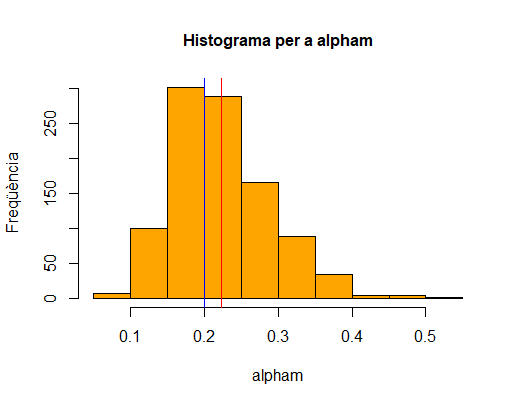
\includegraphics[width=0.45\textwidth]{alpham.png}
  }
  \hfill
  \subfigure{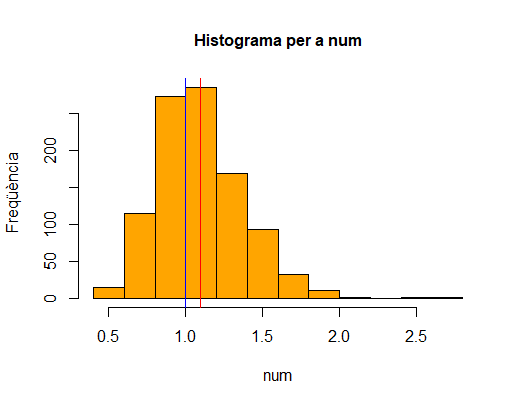
\includegraphics[width=0.45\textwidth]{num.png}
  }
  \caption{Histograma de les freqüències dels valors dels estimadors per a $n=50$, $N=10^3$}
  \label{first}
\end{figure}
  
	Veiem que, tot i que aquests valors s'acosten als valors reals dels paràmetres ($\alpha=0.2,\nu=1$), tenen un cert error que, de fet, podem calcular. Estudiem primer el biaix per a $\hat{\alpha}_m$ i $\hat{\nu}_m$ fent servir la definició però aproximant $E[\hat{\alpha}_m]$ i $E[\hat{\nu}_m]$ per les seves mitjanes aritmètiques $\overline{\hat{\alpha}}_m$ i $\overline{\hat{\nu}}_m$ respectivament.
\begin{align*}
    b(\hat{\alpha}_m)&=\frac{1}{1000}\sum_{i=1}^{1000}\hat{\alpha}_{m_i}-\alpha=0.09404814,\\
    b(\hat{\nu}_m)&=\frac{1}{1000}\sum_{i=1}^{1000}\hat{\nu}_{m_i}-\nu=0.02326543.
\end{align*}
Els errors quadràtics mitjans i les seves arrels respectives seran:
\begin{align*}
    MSE(\hat{\alpha}_m)&=\frac{1}{1000}\sum_{i=1}^{1000}(\hat{\alpha}_{m_i}-\alpha)^2=0.004992216,\\
    RMSE(\hat{\alpha}_m)&=\sqrt{MSE(\hat{\alpha}_m)}=0.07065562,\\
    MSE(\hat{\nu}_m)&=\frac{1}{1000}\sum_{i=1}^{1000}(\hat{\nu}_{m_i}-\nu)^2=0.08650092,\\
    RMSE(\hat{\nu}_m)&=\sqrt{MSE(\hat{\nu}_m)}=0.2941104.
\end{align*}
%%Tots els errors i biaixos igual es podrien posar junts en una taula que potser aixi com esta ara queda massa totxo i al banquer no li agrada... 
Veiem que el RMSE és major per a $\nu$ que per a $\alpha$, però el valor real de nu és cinc vegades major que el d'alpha, pel que podem deduir que tenen un error relatiu semblant. %eredactar-ho millor potser xD

A continuació, repetim els càlculs per a mides mostrals més grans i nombres de simulació més grans. Podem veure els resultats recollits a les taules \ref{globalnu} i \ref{globalalpha}.

\begin{table}[h]
\centering
\caption{Resultats del càlcul de l'estimador $\hat{\nu}_m$ amb diferents mides mostrals i nombres de simulació}\vspace{0.3cm}
\begin{tabular}{|c|c|c|c|c|c|}
\hline
N                    & n   & $\overline{\hat{\nu}_m}$& $b(\hat{\nu}_m)$ & $RMSE(\hat{\nu}_m)$  & $\sqrt{Var(\hat{\nu}_m)}$ \\ \hline
$10^5$                  & 50  & 1.0898 &0.0898& 0.2936  & 0.2795   \\ \hline
$10^4$                   & 50  & 1.0886 &0.0886& 0.2926  & 0.2788   \\ \hline
\multirow{3}{*}{$10^3$ } & 50  & 1.0940 &0.0940& 0.2941  & 0.2787   \\ \cline{2-6} 
                     & 100 & 1.0427 &0.0427& 0.1985  & 0.1939   \\ \cline{2-6} 
                     & 500 & 1.0075 &0.0075& 0.0893 & 0.0890   \\ \hline
\end{tabular}
\label{globalnu}
\end{table}

\begin{table}[h]
\centering
\caption{Resultats del càlcul de l'estimador $\hat{\alpha}_m$ amb diferents mides mostrals i nombres de simulació}\vspace{0.3cm}
\begin{tabular}{|c|c|c|c|c|c|}
\hline
N                    & n   & $\overline{\hat{\alpha}_m}$    &$b(\hat{\alpha}_m)$& $RMSE(\hat{\alpha}_m)$ & $\sqrt{Var(\hat{\alpha}_m)}$ \\ \hline
$10^5$                  & 50  &  0.2225 &0.0225& 0.0697 & 0.0660 \\ \hline
$10^4$                   & 50  &  0.2224 &0.0224& 0.0700 & 0.0663 \\ \hline
\multirow{3}{*}{$10^3$ } & 50  &  0.2233 &0.0233& 0.0707 & 0.0667 \\ \cline{2-6} 
                     & 100 &  0.2113 &0.0113& 0.0462 & 0.0448 \\ \cline{2-6} 
                     & 500 &  0.2021 &0.0021& 0.0207 & 0.0205 \\ \hline
\end{tabular}
\label{globalalpha}
\end{table}

Veiem que, com era d'esperar, en augmentar el nombre d'experiments $N$, el biaix, l'error quadràtic mitjà i la variància d'ambdós estimadors no varien gaire. Això ens indica que hem pres prou quantitat de mostres i que la substitució del valor esperat per la mitjana aritmètica en calcular el biaix, el MSE i la variància és una aproximació prou bona. 

En canvi, aquests valors sí que disminueixen en gran mesura quan augmentem la mida de la mostra. Això ho podem veure en els gràfics de la figura \ref{comparar}. Aquests gràfics són de l'estimador $\hat{\nu}_\text{mom}$, però els gràfics de $\hat{\alpha}_\text{mom}$ tenen la mateixa forma. En augmentar la mida de les mostres, el biaix és més petit i la mitjana dels valors dels estimadors s'apropen al valor real del paràmetre ---com indica l'acostament de les línies blava i vermella---. Per aquest fenomen diem que els estimadors són asimptòticament no esbiaixats. A més a més veiem com clarament en augmentar la mida de la mostra, l'amplada de la distribució dels valors de l'estimador és fa molt més petita (la variància és menor), i el pic al voltant del valor real del paràmetre és molt més pronunciat. Com que els estimadors són asimptòticament no esbiaixats i la variància tendeix a 0 quan $n$ creix, diem que els estimadors són consistents.
%potser faltaria comentar que li passa a la variancia/biaix quan augmentem la mostra. Anar amb compte que el biaix és de cada experiment, no de la mitjana. De fet crec que estaria bé fer el càlcul de la desviació estàndard i relacionar-ho amb l'amplada (peak) de la distribució
%Diria que també s'hauria de comentar que la mitjana dels valors de nu per a n=500 es molt més exaca que la de alpha.
\begin{figure}[!ht]
     \subfigure{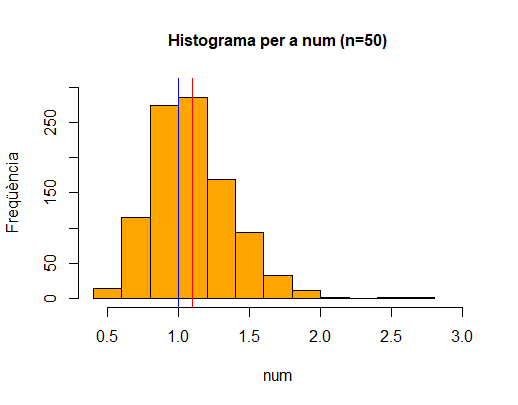
\includegraphics[width=0.50\textwidth]{num50.png}
     }
     \hfill
     \subfigure{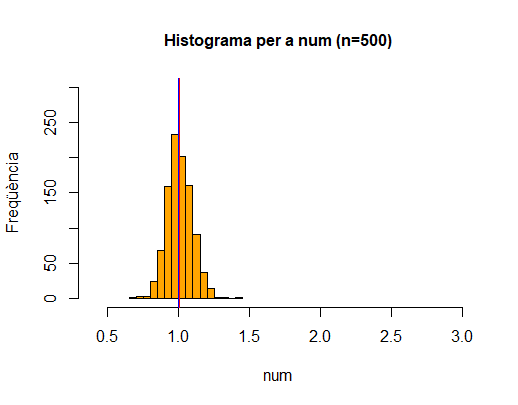
\includegraphics[width=0.50\textwidth]{num500.png}
     }
     \caption{Histogrames de les freqüències dels valors de l'estimador $\nu_m$ per a $N=10^3$, $n=50$ (esquerra) i $n=500$ (dreta).}
     \label{comparar}
  \end{figure}



\subsection{Estimació amb mètozode de màxima versemblança}
Procedim ara a fer el càlcul dels estimadors $\hat{\alpha}_\text{MLE}$ i $\hat{\nu}_\text{MLE}$ mitjançant el mètode de màxima versemblança. Veiem que el càlcul de l'estimador $\hat{\nu} _\text{MLE}$ el podem fer mitjançant la funció \emph{optimize} d'R. De totes maneres, tal com hem mencionat abans, podem fer servir la funció iterativa (\ref{Newton}) pel seu càlcul.
Fent una simulació amb $N=10^3$, $n=50$, $\alpha=0.2$, $\nu=1$, vegem  a la taula \ref{OptimizeNewton} que aquests iterats de Newton convergeixen ràpidament a la solució donada per la funció \emph{optimize}.
\begin{table}[h]
\centering
\caption{Valors de les mitjanes de l'estimador de $\nu$ per als mètode dels moments, funció \emph{optimize} i iterats de Newton.}
\begin{tabular}{|c|c|}
\hline
         & $\overline{\hat{\nu}}$       \\ \hline
Moments  & 1.094048 \\ \hline
Optimize & 1.050163 \\ \hline
Iterat 1 & 1.047203 \\ \hline
Iterat 2 & 1.050160  \\ \hline
Iterat 3 & 1.050163 \\ \hline
\end{tabular}
\label{OptimizeNewton}
\end{table}

Cal notar que el fet que les mitjanes siguin iguals no vol dir que els vectors dels estimadors siguin iguals, però ho hem comprovat amb l'R i, en efecte, coincidien. 
Veiem doncs, que tant la funció \emph{optimize} com el mètode iteratiu són bones opcions per a calcular l'estimador $\hat{\nu_s}$.
Així doncs, realitzem el càlcul dels estimadors per a diferents valors dels paràmetres $\alpha$ i $\nu$ i diferents mides mostrals mitjançant el mètode dels moments i el de màxima versemblança.
\begin{table}[h]
\centering
\caption{Resultats del càlcul d'estimadors amb diferents mides mostrals i nombres de simulació}\vspace{0.3cm}
\begin{tabular}{|c|c|c|c|c|c|c|c|}
\hline
N                    & n   & $\overline{\hat{\nu}_s}$& $b(\overline{\hat{\nu}_s})$ & $RMSE(\overline{\hat{\nu}_s})$  & $\overline{\hat{\alpha}_s}$    & $b(\overline{\hat{\alpha}_s})$ & $RMSE(\overline{\hat{\alpha}_s})$ \\ \hline
$10^5$                  & 50  & 1.0511 &0.0511& 0.2024  & 0.2146 &0.0146& 0.0529   \\ \hline
$10^4$                   & 50  & 1.0502 &0.0502& 0.2013  & 0.2145 &0.0145& 0.0528   \\ \hline
\multirow{3}{*}{$10^3$ } & 50  & 1.0502 &0.0502& 0.2049  & 0.2140 &0.0140& 0.0534   \\ \cline{2-8} 
                     & 100 & 1.0214 &0.0214& 0.1344  & 0.2069 &0.0069& 0.0341   \\ \cline{2-8} 
                     & 500 & 1.0027 &0.0027& 0.0568 & 0.2011 &0.0011& 0.0150   \\ \hline
\end{tabular}
\label{nusalphas}
\end{table}

Els resultats obtinguts i els errors corresponents es poden veure a la taula \ref{nusalphas}. Podem observar fets similars que amb els estimadors pel mètode dels moments. Els resultats no varien en prendre un nombre més gran o més petit de mostres ($N$), però sí que ho fan quan prenem diverses mides mostrals. Com més gran es la mostra, més s'apropen els valors mitjans de $\hat{\nu}_m$ i $\hat{\alpha}_m$ als valors veritables dels paràmetres (estimadors asimptòticament no esbiaixats) i disminueix el seu error quadràtic mitjà (estimadors consistents). A la figura \ref{compararvers} es pot veure que les línies verticals blau i vermella s'acosten en augmentar $n$ (disminueix el biaix) i el pic al voltant de l'1 creix (disminueix la variància).

\begin{figure}[!ht]
     \subfigure{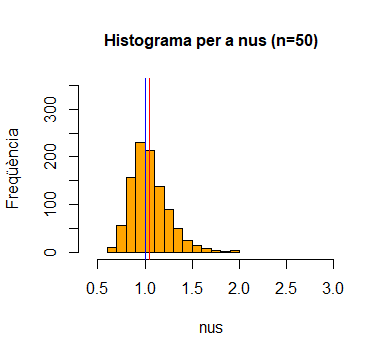
\includegraphics[width=0.50\textwidth]{nus50.png}
     }
     \hfill
     \subfigure{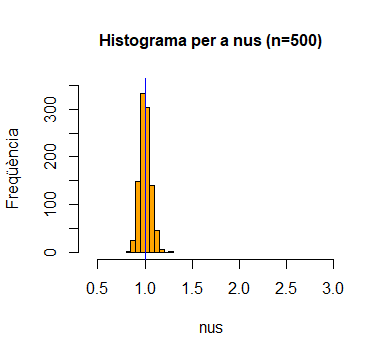
\includegraphics[width=0.50\textwidth]{nus500.png}
     }
     \caption{Histogrames de les freqüències dels valors de l'estimador $\nu_s$ per a $N=10^3$, $n=50$ (esquerra) i $n=500$ (dreta).}
     \label{compararvers}
  \end{figure}

\subsection{Comparació moments-versemblança}
\begin{figure}[htb]
	\sffamily \small \centering
	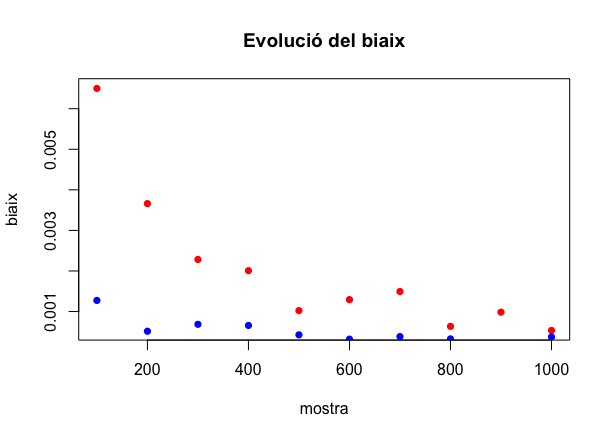
\includegraphics[width = 0.7\textwidth]{biaix.png}
	\caption{Evolució del biaix dels estimadors del paràmetre \( \alpha \) amb la mida de la mostra, fent l'estimació amb \( \alpha = 0.1 \) i \( \nu = 1 \). En blau es mostra el biaix del mètode dels moments, en vermell el de màxima versemblança}
	\label{fig:biaix}
\end{figure}

\begin{figure}[htb]
	\sffamily \small \centering
	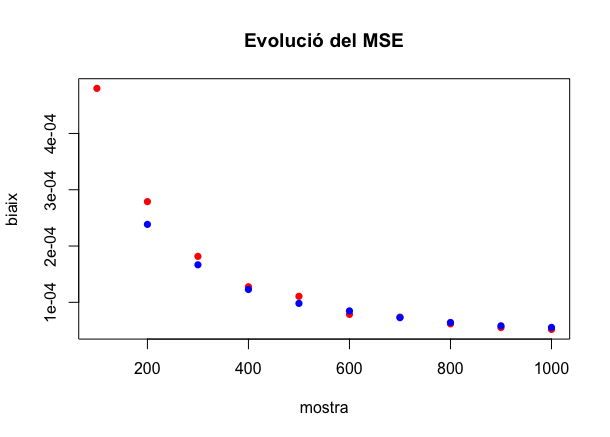
\includegraphics[width = 0.7\textwidth]{mse.png}
	\caption{Evolució del MSE dels estimadors del paràmetre \( \alpha \) amb la mida de la mostra fent l'estimació amb \( \alpha = 0.1 \) i \( \nu = 1 \). En blau es mostra el biaix del mètode dels moments, en vermell el de màxima versemblança}
	\label{fig:mse}
\end{figure}
Podem també comparar els estimadors dels moments i de màxima versemblança entre si. A les taules \ref{globalnu}, \ref{globalalpha} i \ref{comparar} i a les \cref{fig:biaix,fig:mse} es pot veure que el tant el biaix com l'arrel de l'error quadràtic mitjà són en tots els casos (per a diversos $N$, $n$) més petits pels estimadors de màxima versemblança. Això vol dir que aquests són millors estimadors perquè tendeixen cap al valor veritable més ràpidament ---quan n va creixent--- i que estan més concentrats al voltant de la mitjana, tot i que tots dos són bons estimadors, ja que són consistents.

A la taula \ref{tab:resultats}, però, tenim el valor mitjà dels estimadors i el seu RMSE per diversos valors del paràmetre. Veiem que per $\nu=0.5,1,2$ els valors mitjans dels estimadors màxim versemblants són més propers al paràmetre que els dels moments i que el seu error és més petit. Per $\nu=4$ a vegades és més proper el de màxima versemblança i a vegades el dels moments. Per tots dos procediments els valors mitjans dels estimadors tendeixen al paràmetre corresponent quan $n$ es fa gran. Això indica que són asimptòticament no esbiaixats. A més el seu RMSE tendeix cap a 0, pel qual són consistents.


Tal i com veiem a les \cref{fig:biaix,fig:mse}, tant el biaix com el MSE dels dos estimadors (moments i MLE) tendeixen a 0 quan la mida de la mostra creix. Amb això podem concloure amb prou seguretat que tots dos són asimptòticament no esbiaixats i consistents. L'evolució del MSE dels dos estimadors és semblant, però el biaix de l'estimador MLE és més petit a mides petites, per tant podem dir que és millor que l'estimador de moments.  

\section{Conclusions}

Podem concloure que tant els estimadors obtingut pel mètode dels moments com els obtingut pel mètode de màxima versemblança són bones aproximacions dels paràmetres de la distribució gamma per mides mostrals prou grans. Com més gran és la mostra, més petit és el biaix, que tendeix cap a zero quan $n$ tendeix cap a infinit. Per tant els estimadors són asimptòticament no esbiaixats. L'error quadràtic mitjà i la variància també tendeixen cap a zero quan $n$ tendeix cap a infinit. Així doncs aquests dos estimadors són consistents.

La quantitat de mostres que realitzem, però, no influeix gaire en els resultats.

A més podem dir que per $\nu\leq4$ el mètode de màxima versemblança dona millors estimadors que el mètode dels moments, ja que tenen un error quadràtic mitjà més petit.
\newpage

\bibliographystyle{ieeetr}
\bibliography{biblio}


\end{document}

